\documentclass[utf8x, 14pt]{G7-32}

% Настройки стиля ГОСТ 7-32
% Для начала определяем, хотим мы или нет, чтобы рисунки и таблицы нумеровались в пределах раздела, или нам нужна сквозная нумерация.
\EqInChapter % формулы будут нумероваться в пределах раздела
\TableInChapter % таблицы будут нумероваться в пределах раздела
\PicInChapter % рисунки будут нумероваться в пределах раздела
\usepackage{slashbox}

\usepackage[table,xcdraw]{xcolor}

% Добавляем гипертекстовое оглавление в PDF
\usepackage[
bookmarks=true, colorlinks=true, unicode=true,
urlcolor=black,linkcolor=black, anchorcolor=black,
citecolor=black, menucolor=black, filecolor=black,
]{hyperref}

% Изменение начертания шрифта --- после чего выглядит таймсоподобно.
\usepackage{cyrtimespatched}

% графика
\usepackage{graphicx}
\graphicspath{ {./img/} }

% отделять первую строку раздела абзацным отступом
\usepackage{indentfirst} 

% Пакет Tikz
\usepackage{tikz}
\usetikzlibrary{arrows,positioning,shadows}

% Произвольная нумерация списков.
\usepackage{enumerate}

% ячейки в несколько строчек
\usepackage{multirow}

% itemize внутри tabular
\usepackage{paralist,array}

% объявляем новую команду для переноса строки внутри ячейки таблицы
\newcommand{\specialcell}[2][c]{%
	\begin{tabular}[#1]{@{}c@{}}#2\end{tabular}}

\usepackage{tikz}
\usepackage{pgfplots}
\usepackage{pdfpages}
\usepackage{caption}
% \captionsetup[table]{position=top}

\usepackage{listings}
\usepackage{xcolor}

\usepackage{setspace}
\usepackage{tabularx}

\makeatletter
\newcommand{\vhrulefill}[1]
{
	\leavevmode\leaders\hrule\@height#1\hfill \kern\z@
}
\makeatother

\makeatletter
\newcommand{\reportheader}[2]
{
	{\centering
		\bf\huge #1 \\ \bf\Large #2\par
	}
}
\makeatother

% \reportstrattr{имяАтрибута}{значение}
\makeatletter
\newcommand{\reportstrattr}[2]
{
	\large\textbf{#1} & \large{#2} \\\cline{2-2} \\
}
\makeatother

\makeatletter
\newcommand{\reportnumattr}[2]
{
	\large\textbf{#1} & \large{#2} \\ \\
}
\makeatother

% \reportstudent{ФИО}{группа}
\makeatletter
\newcommand{\reportstudent}[2]
{
	\large\textbf{Студент} & #2 & & & ~~ & #1 \\
	\cline{2-2} \cline{4-4} \cline{6-6} \vspace{-4mm} \\
	& & & \large\textsuperscript{(подпись, дата)} & &
	\large\textsuperscript{(Фамилия И.О.)} \\
}
\makeatother

% \reporttutor{ФИО}
\makeatletter
\newcommand{\reporttutor}[1]
{
	\large\textbf{Преподователь} & & & & & #1 \\
	\cline{4-4} \cline{6-6} \vspace{-4mm} \\
	& & & \large\textsuperscript{(подпись, дата)} & &
	\large\textsuperscript{(Фамилия И.О.)} \\
}
\makeatother


% Листинги

\usepackage{listings}
\usepackage{caption}

\usepackage{courier}
\usepackage{wrapfig}

\usepackage{xcolor}
\captionsetup[lstlisting]{singlelinecheck=off, justification=raggedright}

\definecolor{codegreen}{rgb}{0,0.6,0}
\definecolor{codegray}{rgb}{0.5,0.5,0.5}
\definecolor{codepurple}{rgb}{0.58,0,0.82}

\renewcommand{\ttdefault}{cmtt}

%\lstdefinestyle{asm}{
%	language={[x86masm]Assembler},
%	backgroundcolor=\color{white},
%	basicstyle=\footnotesize\ttfamily\bfseries,
%	keywordstyle=\color{blue},
%	stringstyle=\color{red},
%	commentstyle=\color{gray},
%	numbers=left,
%	numberstyle=\tiny,
%	stepnumber=1,
%	numbersep=5pt,
%	frame=single,
%	tabsize=4,
%	captionpos=b,
%	breaklines=true
%}

%\lstdefinestyle{cpp}{
%	language={C++},
%	backgroundcolor=\color{white},
%	basicstyle=\footnotesize\ttfamily\bfseries,
%	keywordstyle=\color{blue},
%	stringstyle=\color{red},
%	commentstyle=\color{gray},
%	numbers=left,
%	numberstyle=\tiny,
%	stepnumber=1,
%	numbersep=5pt,
%	frame=single,
%	tabsize=4,
%	captionpos=b,
%	breaklines=true
%}

% Значения по умолчанию
\lstset{
	% подсветка синтаксиса
	backgroundcolor=\color{white},   
	commentstyle=\color{codegreen},
	keywordstyle=\color{blue},
	numberstyle=\tiny\color{codegray},
	stringstyle=\color{codepurple},
	basicstyle= \footnotesize\ttfamily\bfseries,
	basewidth={.5em,0.5em},
	breakatwhitespace=true,% разрыв строк только на whitespacce
	breaklines=true,       % переносить длинные строки
	% captionpos=b,          % подписи снизу -- вроде не надо
	inputencoding=utf8, %koi8-r,
	numbers=left,          % нумерация слева
	numberstyle=\footnotesize,
	showspaces=false,      % показывать пробелы подчеркиваниями
	showstringspaces=false,
	showtabs=false,        % и табы тоже
	stepnumber=1,
	tabsize=4,              % кому нужны табы по 8 символов?
	frame=single,
	escapeinside={(*}{*)}, %выделение
	literate={а}{{\selectfont\char224}}1
	{б}{{\selectfont\char225}}1
	{в}{{\selectfont\char226}}1
	{г}{{\selectfont\char227}}1
	{д}{{\selectfont\char228}}1
	{е}{{\selectfont\char229}}1
	{ё}{{\"e}}1
	{ж}{{\selectfont\char230}}1
	{з}{{\selectfont\char231}}1
	{и}{{\selectfont\char232}}1
	{й}{{\selectfont\char233}}1
	{к}{{\selectfont\char234}}1
	{л}{{\selectfont\char235}}1
	{м}{{\selectfont\char236}}1
	{н}{{\selectfont\char237}}1
	{о}{{\selectfont\char238}}1
	{п}{{\selectfont\char239}}1
	{р}{{\selectfont\char240}}1
	{с}{{\selectfont\char241}}1
	{т}{{\selectfont\char242}}1
	{у}{{\selectfont\char243}}1
	{ф}{{\selectfont\char244}}1
	{х}{{\selectfont\char245}}1
	{ц}{{\selectfont\char246}}1
	{ч}{{\selectfont\char247}}1
	{ш}{{\selectfont\char248}}1
	{щ}{{\selectfont\char249}}1
	{ъ}{{\selectfont\char250}}1
	{ы}{{\selectfont\char251}}1
	{ь}{{\selectfont\char252}}1
	{э}{{\selectfont\char253}}1
	{ю}{{\selectfont\char254}}1
	{я}{{\selectfont\char255}}1
	{А}{{\selectfont\char192}}1
	{Б}{{\selectfont\char193}}1
	{В}{{\selectfont\char194}}1
	{Г}{{\selectfont\char195}}1
	{Д}{{\selectfont\char196}}1
	{Е}{{\selectfont\char197}}1
	{Ё}{{\"E}}1
	{Ж}{{\selectfont\char198}}1
	{З}{{\selectfont\char199}}1
	{И}{{\selectfont\char200}}1
	{Й}{{\selectfont\char201}}1
	{К}{{\selectfont\char202}}1
	{Л}{{\selectfont\char203}}1
	{М}{{\selectfont\char204}}1
	{Н}{{\selectfont\char205}}1
	{О}{{\selectfont\char206}}1
	{П}{{\selectfont\char207}}1
	{Р}{{\selectfont\char208}}1
	{С}{{\selectfont\char209}}1
	{Т}{{\selectfont\char210}}1
	{У}{{\selectfont\char211}}1
	{Ф}{{\selectfont\char212}}1
	{Х}{{\selectfont\char213}}1
	{Ц}{{\selectfont\char214}}1
	{Ч}{{\selectfont\char215}}1
	{Ш}{{\selectfont\char216}}1
	{Щ}{{\selectfont\char217}}1
	{Ъ}{{\selectfont\char218}}1
	{Ы}{{\selectfont\char219}}1
	{Ь}{{\selectfont\char220}}1
	{Э}{{\selectfont\char221}}1
	{Ю}{{\selectfont\char222}}1
	{Я}{{\selectfont\char223}}1
}

\lstloadlanguages{
	C++
}

% Стиль для псевдокода: строчки обычно короткие, поэтому размер шрифта побольше
\lstdefinestyle{pseudocode}{
	basicstyle=\small,
	keywordstyle=\color{black}\bfseries\underbar,
	language=Pseudocode,
	numberstyle=\footnotesize,
	commentstyle=\footnotesize\it
}

% Стиль для обычного кода: маленький шрифт
\lstdefinestyle{realcode}{
	basicstyle=\scriptsize,
	numberstyle=\footnotesize
}

% Стиль для коротких кусков обычного кода: средний шрифт
\lstdefinestyle{simplecode}{
	basicstyle=\footnotesize,
	numberstyle=\footnotesize
}

% Стиль для BNF
\lstdefinestyle{grammar}{
	basicstyle=\footnotesize,
	numberstyle=\footnotesize,
	stringstyle=\bfseries\ttfamily,
	language=BNF
}

% Определим свой язык для написания псевдокодов на основе Python
\lstdefinelanguage[]{Pseudocode}[]{Python}{
	morekeywords={each,empty,wait,do},% ключевые слова добавлять сюда
	morecomment=[s]{\{}{\}},% комменты {а-ля Pascal} смотрятся нагляднее
	literate=% а сюда добавлять операторы, которые хотите отображать как мат. символы
	{->}{\ensuremath{$\rightarrow$}~}2%
	{<-}{\ensuremath{$\leftarrow$}~}2%
	{:=}{\ensuremath{$\leftarrow$}~}2%
	{<--}{\ensuremath{$\Longleftarrow$}~}2%
}[keywords,comments]

% Свой язык для задания грамматик в BNF
\lstdefinelanguage[]{BNF}[]{}{
	morekeywords={},
	morecomment=[s]{@}{@},
	morestring=[b]",%
	literate=%
	{->}{\ensuremath{$\rightarrow$}~}2%
	{*}{\ensuremath{$^*$}~}2%
	{+}{\ensuremath{$^+$}~}2%
	{|}{\ensuremath{$|$}~}2%
}[keywords,comments,strings]

% Подписи к листингам на русском языке.
\renewcommand\lstlistingname{\cyr\CYRL\cyri\cyrs\cyrt\cyri\cyrn\cyrg}
\renewcommand\lstlistlistingname{\cyr\CYRL\cyri\cyrs\cyrt\cyri\cyrn\cyrg\cyri}



\begin{document}

\frontmatter % выключает нумерацию ВСЕГО; здесь начинаются ненумерованные главы: реферат, введение, глоссарий, сокращения и прочее.

\begin{table}[ht]
	\centering
	\begin{tabular}{|c|p{400pt}|} 
	\hline
		\begin{tabular}[c]{@{}c@{}} 
\includegraphics[scale=0.37]{EmblemBMSTU} \\\end{tabular} &
		\footnotesize\begin{tabular}[c]{@{}c@{}}\textbf{Министерство~науки~и~высшего~образования~Российской~Федерации}\\\textbf{Федеральное~государственное~бюджетное~образовательное~учреждение}\\\textbf{~высшего~образования}\\\textbf{«Московский~государственный~технический~университет}\\\textbf{имени~Н.Э.~Баумана}\\\textbf{(национальный~исследовательский~университет)»}\\\textbf{(МГТУ~им.~Н.Э.~Баумана)}\\\end{tabular}  \\
	\hline
	\end{tabular}
\end{table}
\noindent\rule{\textwidth}{4pt}
\noindent\rule[14pt]{\textwidth}{1pt}
\vspace{-10mm}

\begin{table}[ht]
	\centering
	\begin{tabularx}{\textwidth} {l >{\raggedright\arraybackslash}X }
		\small{ФАКУЛЬТЕТ} & <<Информатика и системы управления>> \\ \cline{2-2} \vspace{-4mm} \\
		\small{КАФЕДРА} & <<Программное обеспечение ЭВМ и информационные технологии>> \\ \cline{2-2}
	\end{tabularx}
\end{table}

\vspace{2cm}
\reportheader{Отчёт}{по лабораторной работе №5}
\vspace{0.5cm}

\begin{table}[h]
	\centering
	\begin{tabularx}{\textwidth} {l >{\raggedright\arraybackslash}X }
		\reportstrattr{Название}{<<Разработка ускорителей вычислений средствами высокоуровневого синтеза>>}
		\reportstrattr{Дисциплина}{<<Архитектура ЭВМ>>}
		\reportnumattr{Вариант}{3}
	\end{tabularx}

	\vspace{3cm}

	\begin{tabularx}{\textwidth} {l c >{\centering\arraybackslash}X c c c }		
		\reportstudent{Клименко А.К.}{ИУ7-55Б}
		\reporttutor{Попов А.Ю.}
	\end{tabularx}
\end{table}

\begin{center}	
	\vfill
	\large \textit {Москва, \the\year}
\end{center}

\thispagestyle {empty}
\pagebreak

\tableofcontents
\pagebreak

\Introduction

\textbf{Целью} данной работы является изучение методики и технологии синтеза
аппаратных устройств ускорения вычислений по описаниям на языках высокого
уровня. В ходе лабораторной работы рассматривается маршрут проектирования
устройств, представленных в виде синтаксических конструкций ЯВУ C/C++,
изучаются принципы работы IDE Xilinx Vitis HLS и методика анализа и отладки
устройств.

Для достижения поставленной цели необходимо выполнить следующие \textbf{задачи}:

\begin{itemize}
	\item pазработать ускоритель вычислений по
индивидуальному заданию;
	\item разработать код для тестирования ускорителя;
	\item
реализовать ускоритель с помощью средств высоко-уровненного синтеза;
	\item
выполнить отладку реализованного ускорителя.
\end{itemize}


\mainmatter % это включает нумерацию глав и секций в документе ниже

\chapter{Функциональная схема разрабатываемой аппаратной
системы}

\begin{figure}
	\centering
	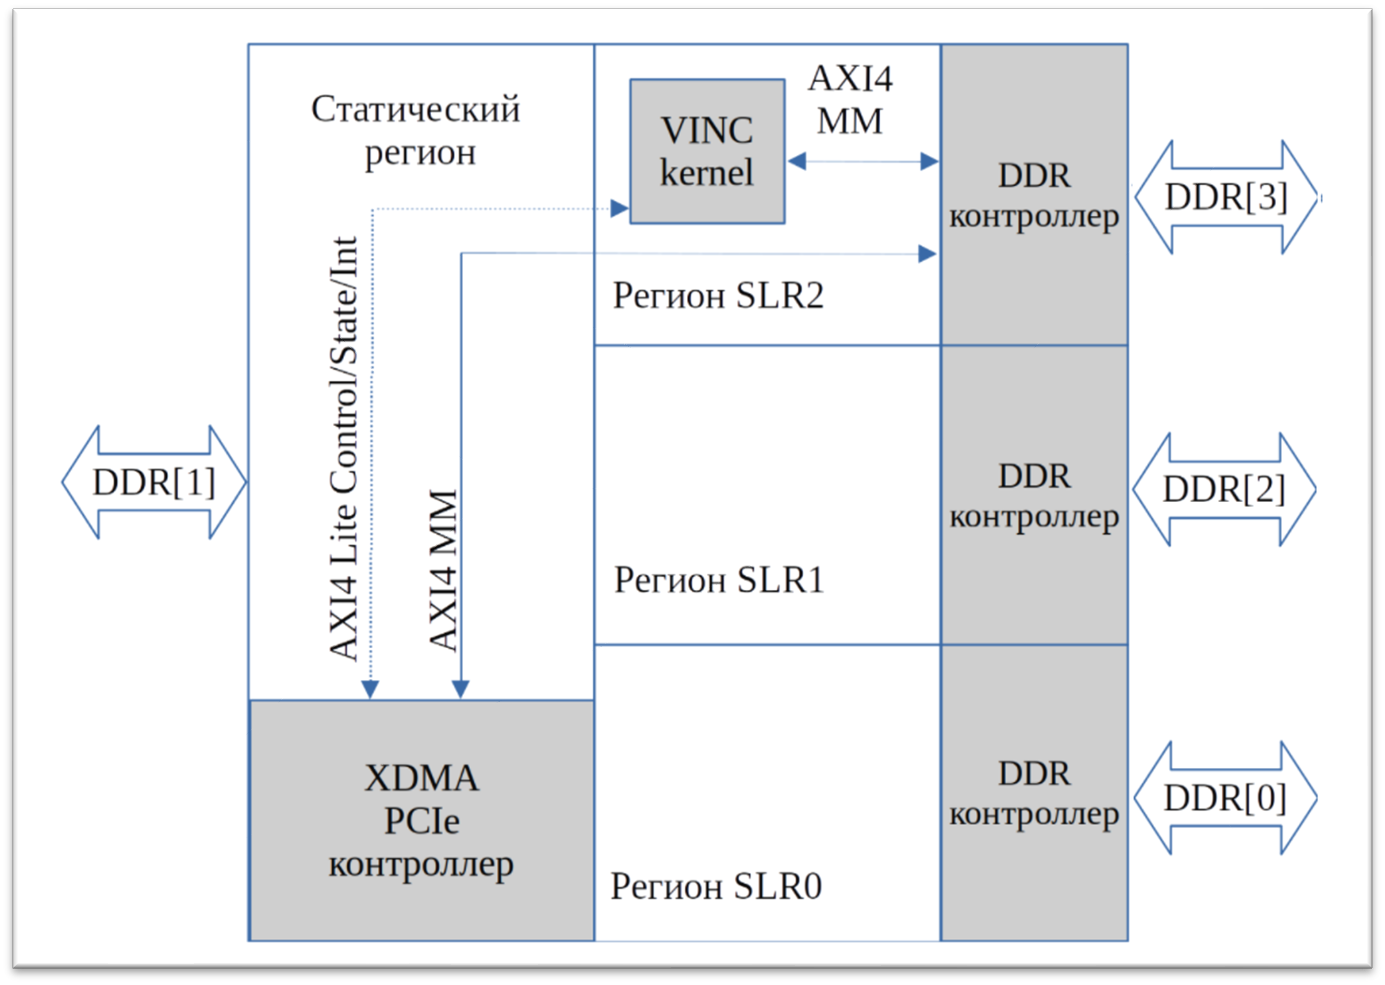
\includegraphics[width=\linewidth]{img/schema.png}
	\caption{Схема аппаратной системы}
\end{figure}

\chapter{Моделирование исходного проекта VINC}

В данном разделе приведены диаграммы, иллюстрирующие процесс рукопожатия и пакетного чтения.

\begin{figure}[ht]
	\centering
	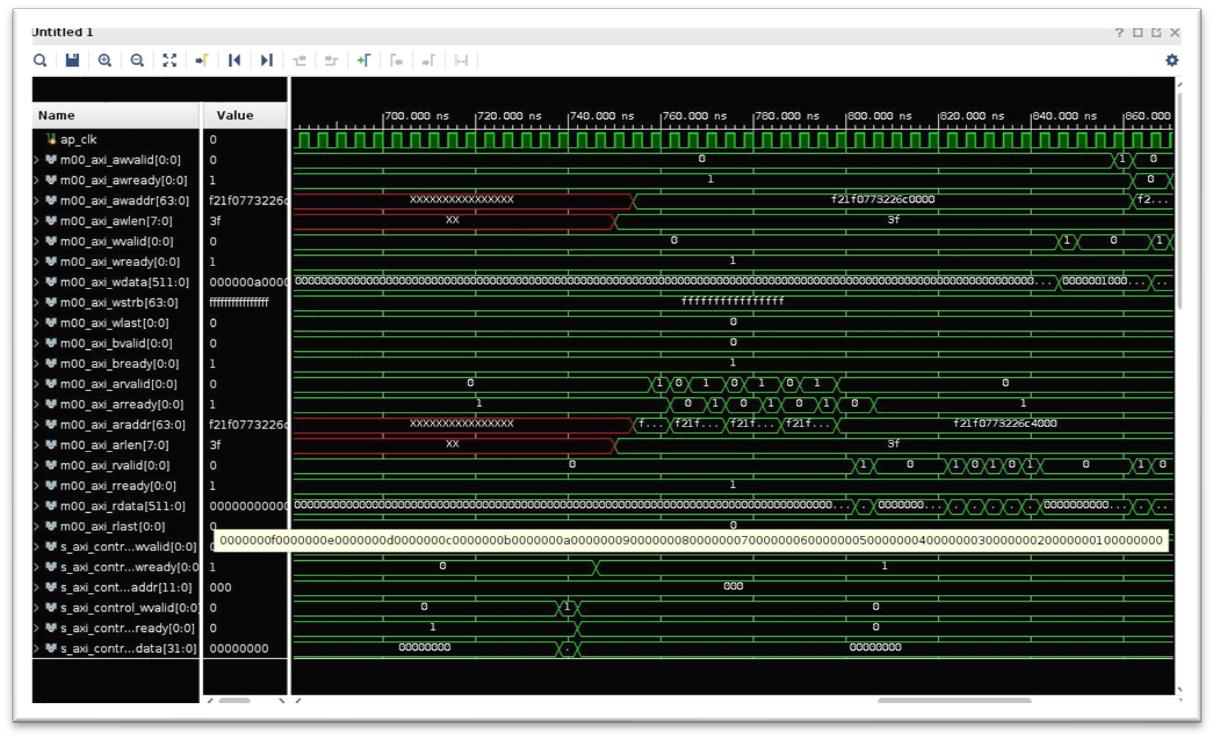
\includegraphics[width=\linewidth]{img/inc-1.png}
	\caption{Транзакция чтения данных вектора на шине AXI4 MM из DDR
памяти}
\end{figure}

\begin{figure}[ht]
	\centering
	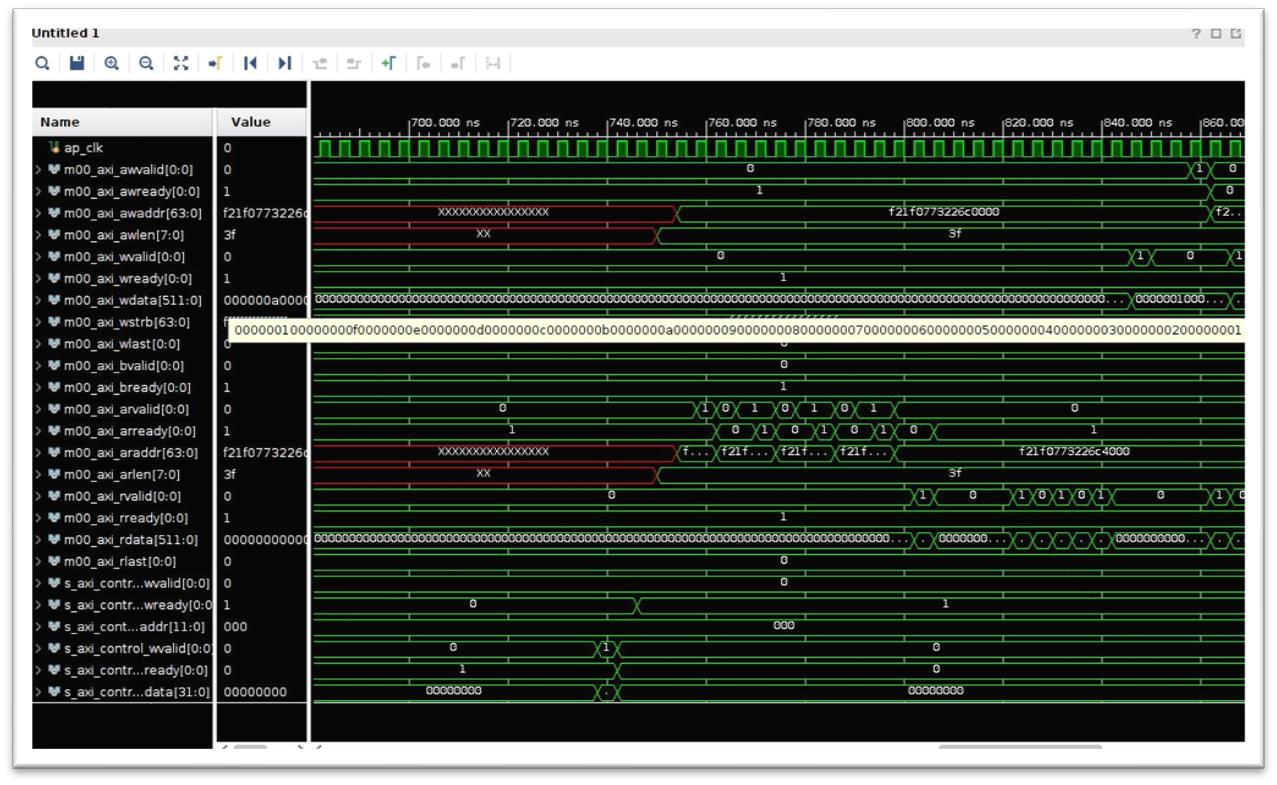
\includegraphics[width=\linewidth]{img/inc-2.png}
	\caption{Транзакция записи результата инкремента данных на шине AXI4
MM}
\end{figure}

\begin{figure}[ht]
	\centering
	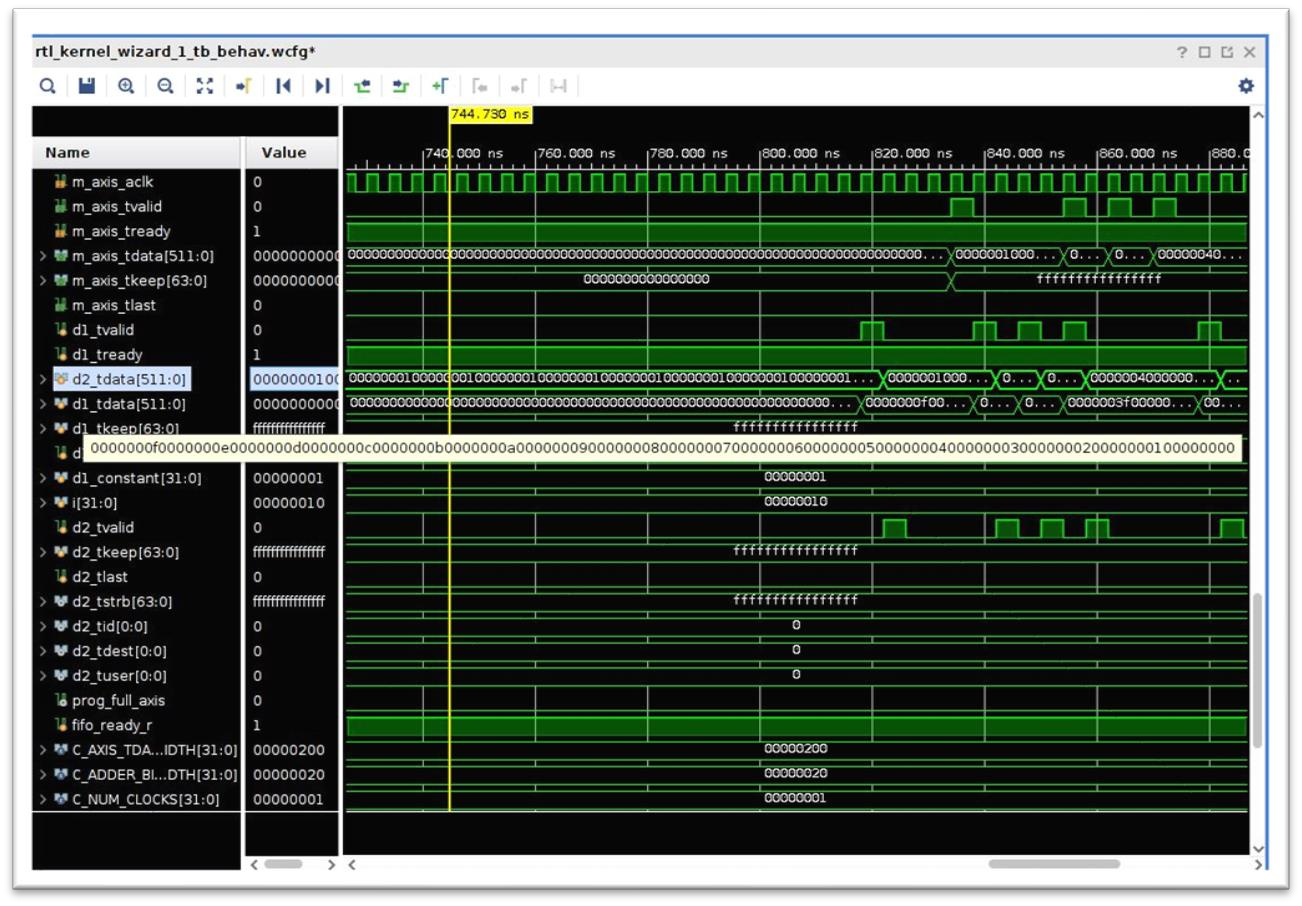
\includegraphics[width=\linewidth]{img/inc-3.png}
	\caption{Инкремент данных}
\end{figure}

\chapter{Моделирование измененного проекта VINC}

Изменим модуль \texttt{rtl\_kernel\_wizard\_2\_example\_adder.v}, чтобы
ускоритель выполнял предложенную функцию:

\begin{equation}
	R[i] = (A[i] - 1) * 4
\end{equation}

Ниже представлен фрагмент листинга кода.

\begin{lstlisting}[language=Pseudocode,caption=Листинг изменённой функции]
always @(posedge s_axis_aclk) begin
  for (i = 0; i < LP_NUM_LOOPS; i = i + 1) begin
    d2_tdata[i*C_ADDER_BIT_WIDTH+:C_ADDER_BIT_WIDTH] <= (d1_tdata[C_ADDER_BIT_WIDTH*i+:C_ADDER_BIT_WIDTH] - 1) * 4;
  end
end
\end{lstlisting}

\begin{figure}[ht]
	\centering
	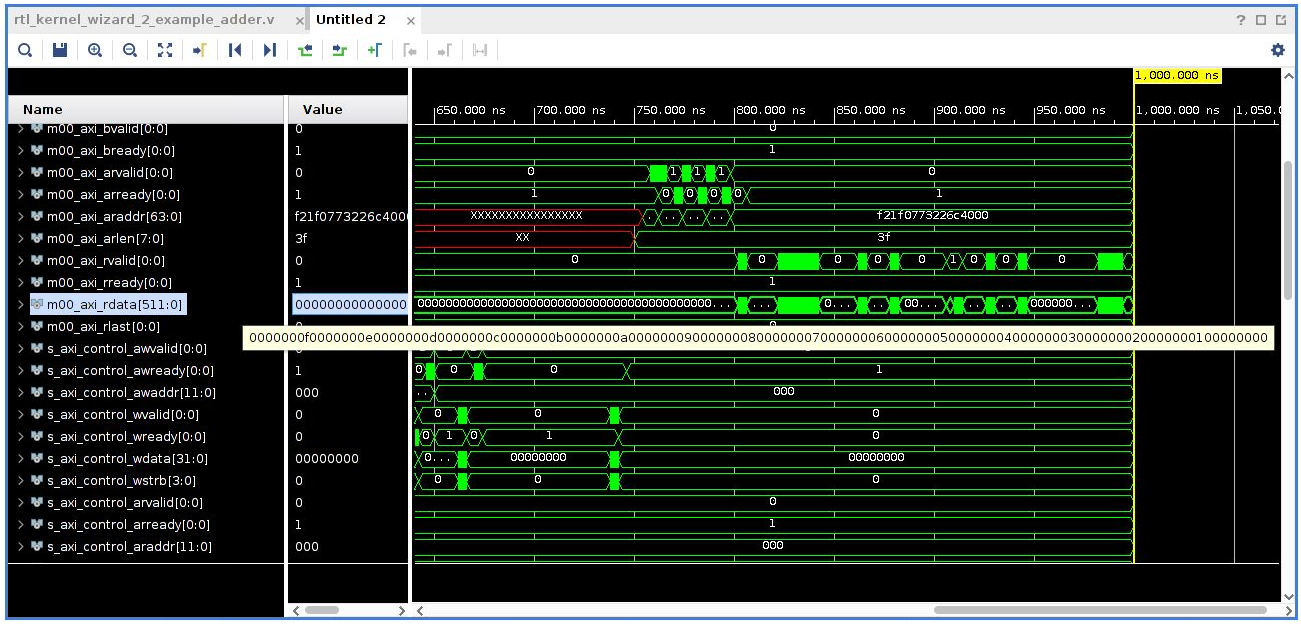
\includegraphics[width=\linewidth]{img/mod-1.png}
	\caption{Транзакция чтения}
\end{figure}

\begin{figure}[ht]
	\centering
	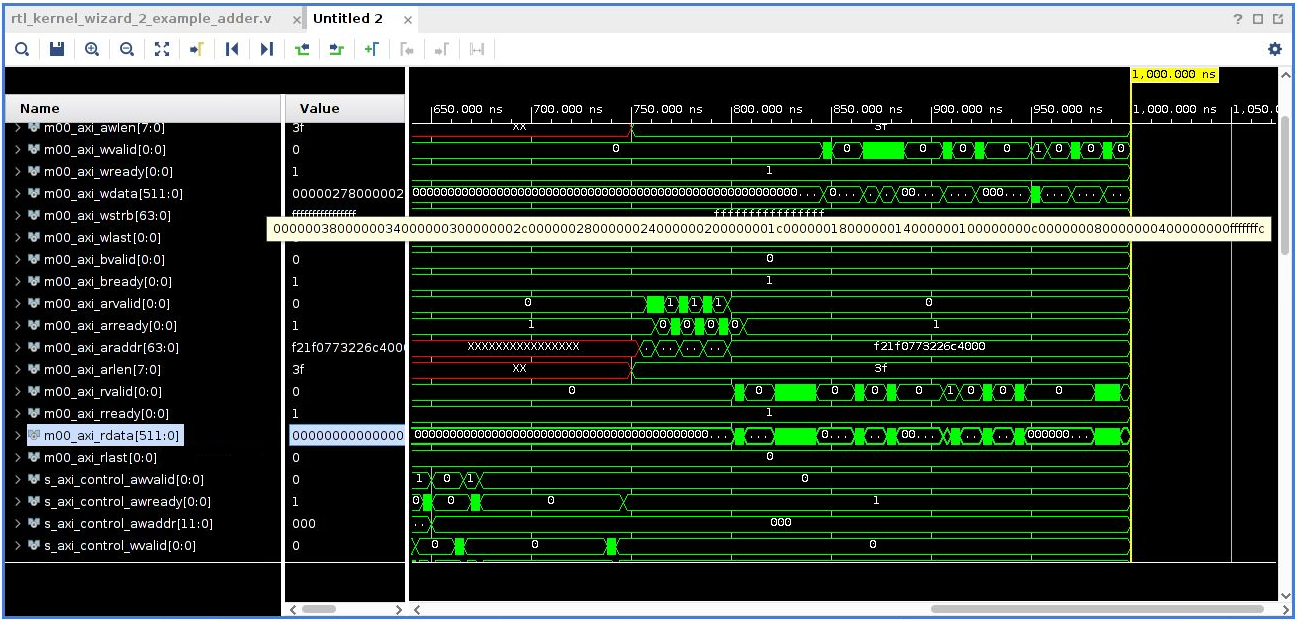
\includegraphics[width=\linewidth]{img/mod-2.png}
	\caption{Транзакция записи}
\end{figure}

\begin{figure}[ht]
	\centering
	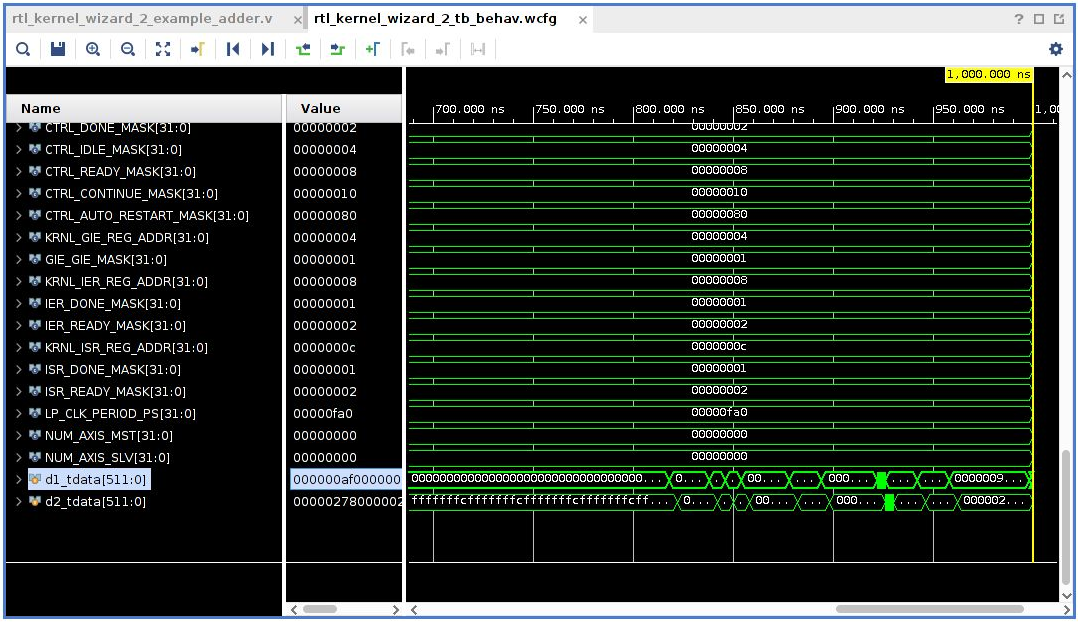
\includegraphics[width=\linewidth]{img/mod-3.png}
	\caption{Изменение данных в модуле}
\end{figure}

\clearpage

\section{Конфигурационный файл линковки}

\lstset{
	frame=none,
	numbers=none,
	breaklines=true
}

\begin{lstlisting}
[connectivity]
nk=rtl_kernel_wizard_2:1:vinc0
slr=vinc0:SLR1
sp=vinc0.m00_axi:DDR[2]

[vivado]
prop=run.impl_1.STEPS.OPT_DESIGN.ARGS.DIRECTIVE=Explore
prop=run.impl_1.STEPS.PLACE_DESIGN.ARGS.DIRECTIVE=Explore
prop=run.impl_1.STEPS.PHYS_OPT_DESIGN.IS_ENABLED=true
prop=run.impl_1.STEPS.PHYS_OPT_DESIGN.ARGS.DIRECTIVE=AggressiveExplore
prop=run.impl_1.STEPS.ROUTE_DESIGN.ARGS.DIRECTIVE=Explore
\end{lstlisting}

\section{Содержимое файла xclbin.info}

\begin{lstlisting}
       Build Date: 2020-11-16 00:19:11
Hash ID: 77d5484b5c4daa691a7f78235053fb036829b1e9
==================================================
xclbin Information
------------------
Generated by:           v++ (2020.2) on 2020-11-18-05:13:29
Version:                2.8.743
Kernels:                rtl_kernel_wizard_2
Signature:              
Content:                Bitstream
UUID (xclbin):          fab9772d-552c-4009-9fa0-8e2dc8ad29e4
Sections:               DEBUG_IP_LAYOUT, BITSTREAM, MEM_TOPOLOGY,
IP_LAYOUT, CONNECTIVITY, CLOCK_FREQ_TOPOLOGY, BUILD_METADATA, 
EMBEDDED_METADATA, SYSTEM_METADATA, 
GROUP_CONNECTIVITY, GROUP_TOPOLOGY
==================================================
Hardware Platform (Shell) Information
-------------------------------------
Vendor:                 xilinx
Board:                  u200
Name:                   xdma
Version:                201830.2
Generated Version:      Vivado 2018.3 (SW Build: 2568420)
Created:                Tue Jun 25 06:55:20 2019
FPGA Device:            xcu200
Board Vendor:           xilinx.com
Board Name:             xilinx.com:au200:1.0
Board Part:             xilinx.com:au200:part0:1.0
Platform VBNV:          xilinx_u200_xdma_201830_2
Static UUID:            c102e7af-b2b8-4381-992b-9a00cc3863eb
Feature ROM TimeStamp:  1561465320

Clocks
------
Name:      DATA_CLK
Index:     0
Type:      DATA
Frequency: 300 MHz

Name:      KERNEL_CLK
Index:     1
Type:      KERNEL
Frequency: 500 MHz

Memory Configuration
--------------------
Name:         bank0
Index:        0
Type:         MEM_DDR4
Base Address: 0x4000000000
Address Size: 0x400000000
Bank Used:    No

Name:         bank1
Index:        1
Type:         MEM_DDR4
Base Address: 0x5000000000
Address Size: 0x400000000
Bank Used:    No

Name:         bank2
Index:        2
Type:         MEM_DDR4
Base Address: 0x6000000000
Address Size: 0x400000000
Bank Used:    Yes

Name:         bank3
Index:        3
Type:         MEM_DDR4
Base Address: 0x7000000000
Address Size: 0x400000000
Bank Used:    No

Name:         PLRAM[0]
Index:        4
Type:         MEM_DRAM
Base Address: 0x3000000000
Address Size: 0x20000
Bank Used:    No

Name:         PLRAM[1]
Index:        5
Type:         MEM_DRAM
Base Address: 0x3000200000
Address Size: 0x20000
Bank Used:    No

Name:         PLRAM[2]
Index:        6
Type:         MEM_DRAM
Base Address: 0x3000400000
Address Size: 0x20000
Bank Used:    No
==================================================
Kernel: rtl_kernel_wizard_2

Definition
----------
Signature: rtl_kernel_wizard_2 (uint inp_param, int* axi00_ptr0)

Ports
-----
Port:          s_axi_control
Mode:          slave
Range (bytes): 0x1000
Data Width:    32 bits
Port Type:     addressable

Port:          m00_axi
Mode:          master
Range (bytes): 0xFFFFFFFFFFFFFFFF
Data Width:    512 bits
Port Type:     addressable

--------------------------
Instance:        vinc0
Base Address: 0x1800000

Argument:          inp_param
Register Offset:   0x010
Port:              s_axi_control
Memory:            <not applicable>

Argument:          axi00_ptr0
Register Offset:   0x018
Port:              m00_axi
Memory:            bank2 (MEM_DDR4)
==================================================
Generated By
------------
Command:       v++
Version:       2020.2 - 2020-11-18-05:13:29 (SW BUILD: 0)
Command Line:  v++ --config ./Alveo_lab1.cfg --connectivity.nk
rtl_kernel_wizard_2:1:vinc0 --connectivity.slr vinc0:SLR1
--connectivity.sp vinc0.m00_axi:DDR[2] --input_files
./rtl_kernel_wizard_2.xo --link --optimize 0 --output vinc.xclbin
--platform xilinx_u200_xdma_201830_2 --report_level 0 --target hw
--vivado.prop run.impl_1.STEPS.OPT_DESIGN.ARGS.DIRECTIVE=Explore
--vivado.prop run.impl_1.STEPS.PLACE_DESIGN.ARGS.DIRECTIVE=Explore
--vivado.prop run.impl_1.STEPS.PHYS_OPT_DESIGN.IS_ENABLED=true
--vivado.prop run.impl_1.STEPS.PHYS_OPT_DESIGN.ARGS.DIRECTIVE=AggressiveExplore --vivado.prop run.impl_1.STEPS.ROUTE_DESIGN.ARGS.DIRECTIVE=Explore 
Options:       --config ./Alveo_lab1.cfg
--connectivity.nk rtl_kernel_wizard_2:1:vinc0
--connectivity.slr vinc0:SLR1
--connectivity.sp vinc0.m00_axi:DDR[2]
--input_files ./rtl_kernel_wizard_2.xo
--link
--optimize 0
--output vinc.xclbin
--platform xilinx_u200_xdma_201830_2
--report_level 0
--target hw
--vivado.prop run.impl_1.STEPS.OPT_DESIGN.ARGS.DIRECTIVE=Explore
--vivado.prop run.impl_1.STEPS.PLACE_DESIGN.ARGS.DIRECTIVE=Explore
--vivado.prop run.impl_1.STEPS.PHYS_OPT_DESIGN.IS_ENABLED=true
--vivado.prop run.impl_1.STEPS.PHYS_OPT_DESIGN.ARGS.DIRECTIVE=AggressiveExplore
--vivado.prop run.impl_1.STEPS.ROUTE_DESIGN.ARGS.DIRECTIVE=Explore 
==================================================
User Added Key Value Pairs
--------------------------
<empty>
==================================================
\end{lstlisting}

\section{Содержимое файла vinc.log}

\begin{lstlisting}
INFO: [v++ 60-1306] Additional information associated with this v++ link can be found at:
Reports: /iu_home/iu7123/workspace/Alveo_lab1_kernels/vivado_rtl_kernel/rtl_kernel_wizard_2_ex/exports/_x/reports/link
Log files: /iu_home/iu7123/workspace/Alveo_lab1_kernels/vivado_rtl_kernel/rtl_kernel_wizard_2_ex/exports/_x/logs/link
INFO: [v++ 60-1548] Creating build summary session with primary output /iu_home/iu7123/workspace/Alveo_lab1_kernels/vivado_rtl_kernel/rtl_kernel_wizard_2_ex/exports/vinc.xclbin.link_summary, at Mon Oct 11 23:09:22 2021
INFO: [v++ 60-1316] Initiating connection to rulecheck server, at Mon Oct 11 23:09:24 2021
INFO: [v++ 60-1315] Creating rulecheck session with output '/iu_home/iu7123/workspace/Alveo_lab1_kernels/vivado_rtl_kernel/rtl_kernel_wizard_2_ex/exports/_x/reports/link/v++_link_vinc_guidance.html', at Mon Oct 11 23:09:43 2021
INFO: [v++ 60-895]   Target platform: /opt/xilinx/platforms/xilinx_u200_xdma_201830_2/xilinx_u200_xdma_201830_2.xpfm
INFO: [v++ 60-1578]   This platform contains Device Support Archive '/opt/xilinx/platforms/xilinx_u200_xdma_201830_2/hw/xilinx_u200_xdma_201830_2.dsa'
INFO: [v++ 74-74] Compiler Version string: 2020.2
INFO: [v++ 60-1302] Platform 'xilinx_u200_xdma_201830_2.xpfm' has been explicitly enabled for this release.
INFO: [v++ 60-629] Linking for hardware target
INFO: [v++ 60-423]   Target device: xilinx_u200_xdma_201830_2
INFO: [v++ 60-1332] Run 'run_link' status: Not started
INFO: [v++ 60-1443] [23:10:50] Run run_link: Step system_link: Started
INFO: [v++ 60-1453] Command Line: system_link --xo /iu_home/iu7123/workspace/Alveo_lab1_kernels/vivado_rtl_kernel/rtl_kernel_wizard_2_ex/exports/rtl_kernel_wizard_2.xo --config /iu_home/iu7123/workspace/Alveo_lab1_kernels/vivado_rtl_kernel/rtl_kernel_wizard_2_ex/exports/_x/link/int/syslinkConfig.ini --xpfm /opt/xilinx/platforms/xilinx_u200_xdma_201830_2/xilinx_u200_xdma_201830_2.xpfm --target hw --output_dir /iu_home/iu7123/workspace/Alveo_lab1_kernels/vivado_rtl_kernel/rtl_kernel_wizard_2_ex/exports/_x/link/int --temp_dir /iu_home/iu7123/workspace/Alveo_lab1_kernels/vivado_rtl_kernel/rtl_kernel_wizard_2_ex/exports/_x/link/sys_link
INFO: [v++ 60-1454] Run Directory: /iu_home/iu7123/workspace/Alveo_lab1_kernels/vivado_rtl_kernel/rtl_kernel_wizard_2_ex/exports/_x/link/run_link
INFO: [SYSTEM_LINK 60-1316] Initiating connection to rulecheck server, at Mon Oct 11 23:11:08 2021
INFO: [SYSTEM_LINK 82-70] Extracting xo v3 file /iu_home/iu7123/workspace/Alveo_lab1_kernels/vivado_rtl_kernel/rtl_kernel_wizard_2_ex/exports/rtl_kernel_wizard_2.xo
INFO: [SYSTEM_LINK 82-53] Creating IP database /iu_home/iu7123/workspace/Alveo_lab1_kernels/vivado_rtl_kernel/rtl_kernel_wizard_2_ex/exports/_x/link/sys_link/_sysl/.cdb/xd_ip_db.xml
INFO: [SYSTEM_LINK 82-38] [23:11:14] build_xd_ip_db started: /data/Xilinx/Vitis/2020.2/bin/build_xd_ip_db -ip_search 0  -sds-pf /iu_home/iu7123/workspace/Alveo_lab1_kernels/vivado_rtl_kernel/rtl_kernel_wizard_2_ex/exports/_x/link/sys_link/xilinx_u200_xdma_201830_2.hpfm -clkid 0 -ip /iu_home/iu7123/workspace/Alveo_lab1_kernels/vivado_rtl_kernel/rtl_kernel_wizard_2_ex/exports/_x/link/sys_link/iprepo/mycompany_com_kernel_rtl_kernel_wizard_2_1_0,rtl_kernel_wizard_2 -o /iu_home/iu7123/workspace/Alveo_lab1_kernels/vivado_rtl_kernel/rtl_kernel_wizard_2_ex/exports/_x/link/sys_link/_sysl/.cdb/xd_ip_db.xml
INFO: [SYSTEM_LINK 82-37] [23:11:57] build_xd_ip_db finished successfully
Time (s): cpu = 00:00:35 ; elapsed = 00:00:43 . Memory (MB): peak = 1557.895 ; gain = 0.000 ; free physical = 57836 ; free virtual = 295751
INFO: [SYSTEM_LINK 82-51] Create system connectivity graph
INFO: [SYSTEM_LINK 82-102] Applying explicit connections to the system connectivity graph: /iu_home/iu7123/workspace/Alveo_lab1_kernels/vivado_rtl_kernel/rtl_kernel_wizard_2_ex/exports/_x/link/sys_link/cfgraph/cfgen_cfgraph.xml
INFO: [SYSTEM_LINK 82-38] [23:11:57] cfgen started: /data/Xilinx/Vitis/2020.2/bin/cfgen  -nk rtl_kernel_wizard_2:1:vinc0 -slr vinc0:SLR1 -sp vinc0.m00_axi:DDR[2] -dmclkid 0 -r /iu_home/iu7123/workspace/Alveo_lab1_kernels/vivado_rtl_kernel/rtl_kernel_wizard_2_ex/exports/_x/link/sys_link/_sysl/.cdb/xd_ip_db.xml -o /iu_home/iu7123/workspace/Alveo_lab1_kernels/vivado_rtl_kernel/rtl_kernel_wizard_2_ex/exports/_x/link/sys_link/cfgraph/cfgen_cfgraph.xml
INFO: [CFGEN 83-0] Kernel Specs: 
INFO: [CFGEN 83-0]   kernel: rtl_kernel_wizard_2, num: 1  {vinc0}
INFO: [CFGEN 83-0] Port Specs: 
INFO: [CFGEN 83-0]   kernel: vinc0, k_port: m00_axi, sptag: DDR[2]
INFO: [CFGEN 83-0] SLR Specs: 
INFO: [CFGEN 83-0]   instance: vinc0, SLR: SLR1
INFO: [CFGEN 83-2228] Creating mapping for argument vinc0.axi00_ptr0 to DDR[2] for directive vinc0.m00_axi:DDR[2]
INFO: [SYSTEM_LINK 82-37] [23:12:31] cfgen finished successfully
Time (s): cpu = 00:00:33 ; elapsed = 00:00:34 . Memory (MB): peak = 1557.895 ; gain = 0.000 ; free physical = 57870 ; free virtual = 295785
INFO: [SYSTEM_LINK 82-52] Create top-level block diagram
INFO: [SYSTEM_LINK 82-38] [23:12:31] cf2bd started: /data/Xilinx/Vitis/2020.2/bin/cf2bd  --linux --trace_buffer 1024 --input_file /iu_home/iu7123/workspace/Alveo_lab1_kernels/vivado_rtl_kernel/rtl_kernel_wizard_2_ex/exports/_x/link/sys_link/cfgraph/cfgen_cfgraph.xml --ip_db /iu_home/iu7123/workspace/Alveo_lab1_kernels/vivado_rtl_kernel/rtl_kernel_wizard_2_ex/exports/_x/link/sys_link/_sysl/.cdb/xd_ip_db.xml --cf_name dr --working_dir /iu_home/iu7123/workspace/Alveo_lab1_kernels/vivado_rtl_kernel/rtl_kernel_wizard_2_ex/exports/_x/link/sys_link/_sysl/.xsd --temp_dir /iu_home/iu7123/workspace/Alveo_lab1_kernels/vivado_rtl_kernel/rtl_kernel_wizard_2_ex/exports/_x/link/sys_link --output_dir /iu_home/iu7123/workspace/Alveo_lab1_kernels/vivado_rtl_kernel/rtl_kernel_wizard_2_ex/exports/_x/link/int --target_bd pfm_dynamic.bd
INFO: [CF2BD 82-31] Launching cf2xd: cf2xd -linux -trace-buffer 1024 -i /iu_home/iu7123/workspace/Alveo_lab1_kernels/vivado_rtl_kernel/rtl_kernel_wizard_2_ex/exports/_x/link/sys_link/cfgraph/cfgen_cfgraph.xml -r /iu_home/iu7123/workspace/Alveo_lab1_kernels/vivado_rtl_kernel/rtl_kernel_wizard_2_ex/exports/_x/link/sys_link/_sysl/.cdb/xd_ip_db.xml -o dr.xml
INFO: [CF2BD 82-28] cf2xd finished successfully
INFO: [CF2BD 82-31] Launching cf_xsd: cf_xsd -disable-address-gen -bd pfm_dynamic.bd -dn dr -dp /iu_home/iu7123/workspace/Alveo_lab1_kernels/vivado_rtl_kernel/rtl_kernel_wizard_2_ex/exports/_x/link/sys_link/_sysl/.xsd
INFO: [CF2BD 82-28] cf_xsd finished successfully
INFO: [SYSTEM_LINK 82-37] [23:12:51] cf2bd finished successfully
Time (s): cpu = 00:00:15 ; elapsed = 00:00:19 . Memory (MB): peak = 1557.895 ; gain = 0.000 ; free physical = 57841 ; free virtual = 295761
INFO: [v++ 60-1441] [23:12:51] Run run_link: Step system_link: Completed
Time (s): cpu = 00:01:46 ; elapsed = 00:02:02 . Memory (MB): peak = 1721.133 ; gain = 0.000 ; free physical = 57920 ; free virtual = 295835
INFO: [v++ 60-1443] [23:12:51] Run run_link: Step cf2sw: Started
INFO: [v++ 60-1453] Command Line: cf2sw -sdsl /iu_home/iu7123/workspace/Alveo_lab1_kernels/vivado_rtl_kernel/rtl_kernel_wizard_2_ex/exports/_x/link/int/sdsl.dat -rtd /iu_home/iu7123/workspace/Alveo_lab1_kernels/vivado_rtl_kernel/rtl_kernel_wizard_2_ex/exports/_x/link/int/cf2sw.rtd -nofilter /iu_home/iu7123/workspace/Alveo_lab1_kernels/vivado_rtl_kernel/rtl_kernel_wizard_2_ex/exports/_x/link/int/cf2sw_full.rtd -xclbin /iu_home/iu7123/workspace/Alveo_lab1_kernels/vivado_rtl_kernel/rtl_kernel_wizard_2_ex/exports/_x/link/int/xclbin_orig.xml -o /iu_home/iu7123/workspace/Alveo_lab1_kernels/vivado_rtl_kernel/rtl_kernel_wizard_2_ex/exports/_x/link/int/xclbin_orig.1.xml
INFO: [v++ 60-1454] Run Directory: /iu_home/iu7123/workspace/Alveo_lab1_kernels/vivado_rtl_kernel/rtl_kernel_wizard_2_ex/exports/_x/link/run_link
INFO: [v++ 60-1441] [23:13:14] Run run_link: Step cf2sw: Completed
Time (s): cpu = 00:00:19 ; elapsed = 00:00:22 . Memory (MB): peak = 1721.133 ; gain = 0.000 ; free physical = 58006 ; free virtual = 295921
INFO: [v++ 60-1443] [23:13:14] Run run_link: Step rtd2_system_diagram: Started
INFO: [v++ 60-1453] Command Line: rtd2SystemDiagram
INFO: [v++ 60-1454] Run Directory: /iu_home/iu7123/workspace/Alveo_lab1_kernels/vivado_rtl_kernel/rtl_kernel_wizard_2_ex/exports/_x/link/run_link
INFO: [v++ 60-1441] [23:13:26] Run run_link: Step rtd2_system_diagram: Completed
Time (s): cpu = 00:00:00.01 ; elapsed = 00:00:13 . Memory (MB): peak = 1721.133 ; gain = 0.000 ; free physical = 57220 ; free virtual = 295135
INFO: [v++ 60-1443] [23:13:26] Run run_link: Step vpl: Started
INFO: [v++ 60-1453] Command Line: vpl -t hw -f xilinx_u200_xdma_201830_2 --remote_ip_cache /iu_home/iu7123/workspace/Alveo_lab1_kernels/vivado_rtl_kernel/rtl_kernel_wizard_2_ex/exports/.ipcache --output_dir /iu_home/iu7123/workspace/Alveo_lab1_kernels/vivado_rtl_kernel/rtl_kernel_wizard_2_ex/exports/_x/link/int --log_dir /iu_home/iu7123/workspace/Alveo_lab1_kernels/vivado_rtl_kernel/rtl_kernel_wizard_2_ex/exports/_x/logs/link --report_dir /iu_home/iu7123/workspace/Alveo_lab1_kernels/vivado_rtl_kernel/rtl_kernel_wizard_2_ex/exports/_x/reports/link --config /iu_home/iu7123/workspace/Alveo_lab1_kernels/vivado_rtl_kernel/rtl_kernel_wizard_2_ex/exports/_x/link/int/vplConfig.ini -k /iu_home/iu7123/workspace/Alveo_lab1_kernels/vivado_rtl_kernel/rtl_kernel_wizard_2_ex/exports/_x/link/int/kernel_info.dat --webtalk_flag Vitis --temp_dir /iu_home/iu7123/workspace/Alveo_lab1_kernels/vivado_rtl_kernel/rtl_kernel_wizard_2_ex/exports/_x/link --no-info --iprepo /iu_home/iu7123/workspace/Alveo_lab1_kernels/vivado_rtl_kernel/rtl_kernel_wizard_2_ex/exports/_x/link/int/xo/ip_repo/mycompany_com_kernel_rtl_kernel_wizard_2_1_0 --messageDb /iu_home/iu7123/workspace/Alveo_lab1_kernels/vivado_rtl_kernel/rtl_kernel_wizard_2_ex/exports/_x/link/run_link/vpl.pb /iu_home/iu7123/workspace/Alveo_lab1_kernels/vivado_rtl_kernel/rtl_kernel_wizard_2_ex/exports/_x/link/int/dr.bd.tcl
INFO: [v++ 60-1454] Run Directory: /iu_home/iu7123/workspace/Alveo_lab1_kernels/vivado_rtl_kernel/rtl_kernel_wizard_2_ex/exports/_x/link/run_link

****** vpl v2020.2 (64-bit)
**** SW Build (by xbuild) on 2020-11-18-05:13:29
** Copyright 1986-2020 Xilinx, Inc. All Rights Reserved.

INFO: [VPL 60-839] Read in kernel information from file '/iu_home/iu7123/workspace/Alveo_lab1_kernels/vivado_rtl_kernel/rtl_kernel_wizard_2_ex/exports/_x/link/int/kernel_info.dat'.
INFO: [VPL 74-74] Compiler Version string: 2020.2
INFO: [VPL 60-423]   Target device: xilinx_u200_xdma_201830_2
INFO: [VPL 60-1032] Extracting hardware platform to /iu_home/iu7123/workspace/Alveo_lab1_kernels/vivado_rtl_kernel/rtl_kernel_wizard_2_ex/exports/_x/link/vivado/vpl/.local/hw_platform
WARNING: /data/Xilinx/Vitis/2020.2/tps/lnx64/jre9.0.4 does not exist.
[23:21:34] Run vpl: Step create_project: RUNNING...
[23:21:24] Run vpl: Step create_project: Started
Creating Vivado project.
[23:22:03] Run vpl: Step create_project: Completed
[23:22:03] Run vpl: Step create_bd: Started
[23:24:20] Run vpl: Step create_bd: RUNNING...
[23:29:37] Run vpl: Step create_bd: RUNNING...
[23:31:34] Run vpl: Step create_bd: RUNNING...
[23:33:35] Run vpl: Step create_bd: RUNNING...
[23:35:19] Run vpl: Step create_bd: RUNNING...
[23:37:12] Run vpl: Step create_bd: RUNNING...
[23:38:59] Run vpl: Step create_bd: RUNNING...
[23:39:15] Run vpl: Step create_bd: Completed
[23:39:15] Run vpl: Step update_bd: Started
[23:39:20] Run vpl: Step update_bd: Completed
[23:39:20] Run vpl: Step generate_target: Started
[23:42:09] Run vpl: Step generate_target: RUNNING...
[23:44:02] Run vpl: Step generate_target: RUNNING...
[23:45:27] Run vpl: Step generate_target: RUNNING...
[23:47:17] Run vpl: Step generate_target: RUNNING...
[23:48:53] Run vpl: Step generate_target: RUNNING...
[23:50:38] Run vpl: Step generate_target: RUNNING...
[23:52:22] Run vpl: Step generate_target: RUNNING...
[23:54:10] Run vpl: Step generate_target: Completed
[23:54:10] Run vpl: Step config_hw_runs: Started
[23:54:15] Run vpl: Step generate_target: RUNNING...
[23:56:20] Run vpl: Step config_hw_runs: RUNNING...
[23:56:31] Run vpl: Step config_hw_runs: Completed
[23:56:31] Run vpl: Step synth: Started
[23:59:27] Block-level synthesis in progress, 0 of 66 jobs complete, 8 jobs running.
[00:00:09] Block-level synthesis in progress, 0 of 66 jobs complete, 8 jobs running.
[00:01:04] Block-level synthesis in progress, 0 of 66 jobs complete, 8 jobs running.
[00:01:46] Block-level synthesis in progress, 0 of 66 jobs complete, 8 jobs running.
[00:02:27] Block-level synthesis in progress, 0 of 66 jobs complete, 8 jobs running.
[00:03:07] Block-level synthesis in progress, 0 of 66 jobs complete, 8 jobs running.
[00:03:51] Block-level synthesis in progress, 0 of 66 jobs complete, 8 jobs running.
[00:04:32] Block-level synthesis in progress, 0 of 66 jobs complete, 8 jobs running.
[00:05:07] Block-level synthesis in progress, 0 of 66 jobs complete, 8 jobs running.
[00:05:47] Block-level synthesis in progress, 0 of 66 jobs complete, 8 jobs running.
[00:06:34] Block-level synthesis in progress, 0 of 66 jobs complete, 8 jobs running.
[00:07:19] Block-level synthesis in progress, 0 of 66 jobs complete, 8 jobs running.
[00:08:09] Block-level synthesis in progress, 2 of 66 jobs complete, 6 jobs running.
[00:08:54] Block-level synthesis in progress, 6 of 66 jobs complete, 2 jobs running.
[00:09:30] Block-level synthesis in progress, 6 of 66 jobs complete, 4 jobs running.
[00:10:08] Block-level synthesis in progress, 6 of 66 jobs complete, 7 jobs running.
[00:10:52] Block-level synthesis in progress, 7 of 66 jobs complete, 7 jobs running.
[00:11:30] Block-level synthesis in progress, 7 of 66 jobs complete, 7 jobs running.
[00:12:22] Block-level synthesis in progress, 8 of 66 jobs complete, 6 jobs running.
[00:13:01] Block-level synthesis in progress, 8 of 66 jobs complete, 7 jobs running.
[00:13:50] Block-level synthesis in progress, 8 of 66 jobs complete, 8 jobs running.
[00:14:30] Block-level synthesis in progress, 8 of 66 jobs complete, 8 jobs running.
[00:15:09] Block-level synthesis in progress, 8 of 66 jobs complete, 8 jobs running.
[00:15:51] Block-level synthesis in progress, 8 of 66 jobs complete, 8 jobs running.
[00:16:41] Block-level synthesis in progress, 8 of 66 jobs complete, 8 jobs running.
[00:17:21] Block-level synthesis in progress, 8 of 66 jobs complete, 8 jobs running.
[00:18:06] Block-level synthesis in progress, 9 of 66 jobs complete, 7 jobs running.
[00:18:47] Block-level synthesis in progress, 11 of 66 jobs complete, 5 jobs running.
[00:19:35] Block-level synthesis in progress, 13 of 66 jobs complete, 3 jobs running.
[00:20:15] Block-level synthesis in progress, 14 of 66 jobs complete, 5 jobs running.
[00:20:56] Block-level synthesis in progress, 14 of 66 jobs complete, 7 jobs running.
[00:21:34] Block-level synthesis in progress, 14 of 66 jobs complete, 8 jobs running.
[00:22:29] Block-level synthesis in progress, 15 of 66 jobs complete, 7 jobs running.
[00:23:06] Block-level synthesis in progress, 16 of 66 jobs complete, 6 jobs running.
[00:23:55] Block-level synthesis in progress, 16 of 66 jobs complete, 6 jobs running.
[00:24:33] Block-level synthesis in progress, 16 of 66 jobs complete, 8 jobs running.
[00:25:11] Block-level synthesis in progress, 16 of 66 jobs complete, 8 jobs running.
[00:25:50] Block-level synthesis in progress, 16 of 66 jobs complete, 8 jobs running.
[00:26:28] Block-level synthesis in progress, 16 of 66 jobs complete, 8 jobs running.
[00:27:11] Block-level synthesis in progress, 16 of 66 jobs complete, 8 jobs running.
[00:27:53] Block-level synthesis in progress, 16 of 66 jobs complete, 8 jobs running.
[00:28:30] Block-level synthesis in progress, 16 of 66 jobs complete, 8 jobs running.
[00:29:15] Block-level synthesis in progress, 17 of 66 jobs complete, 7 jobs running.
[00:29:52] Block-level synthesis in progress, 17 of 66 jobs complete, 7 jobs running.
[00:30:33] Block-level synthesis in progress, 18 of 66 jobs complete, 6 jobs running.
[00:31:10] Block-level synthesis in progress, 18 of 66 jobs complete, 7 jobs running.
[00:32:01] Block-level synthesis in progress, 19 of 66 jobs complete, 6 jobs running.
[00:32:40] Block-level synthesis in progress, 19 of 66 jobs complete, 7 jobs running.
[00:33:48] Block-level synthesis in progress, 19 of 66 jobs complete, 8 jobs running.
[00:34:28] Block-level synthesis in progress, 21 of 66 jobs complete, 6 jobs running.
[00:35:10] Block-level synthesis in progress, 21 of 66 jobs complete, 6 jobs running.
[00:35:53] Block-level synthesis in progress, 21 of 66 jobs complete, 8 jobs running.
[00:36:32] Block-level synthesis in progress, 22 of 66 jobs complete, 7 jobs running.
[00:37:22] Block-level synthesis in progress, 22 of 66 jobs complete, 7 jobs running.
[00:38:01] Block-level synthesis in progress, 22 of 66 jobs complete, 8 jobs running.
[00:38:41] Block-level synthesis in progress, 22 of 66 jobs complete, 8 jobs running.
[00:39:33] Block-level synthesis in progress, 22 of 66 jobs complete, 8 jobs running.
[00:40:15] Block-level synthesis in progress, 22 of 66 jobs complete, 8 jobs running.
[00:41:18] Block-level synthesis in progress, 23 of 66 jobs complete, 7 jobs running.
[00:42:31] Block-level synthesis in progress, 23 of 66 jobs complete, 8 jobs running.
[00:43:11] Block-level synthesis in progress, 25 of 66 jobs complete, 6 jobs running.
[00:43:57] Block-level synthesis in progress, 25 of 66 jobs complete, 6 jobs running.
[00:44:38] Block-level synthesis in progress, 25 of 66 jobs complete, 8 jobs running.
[00:45:23] Block-level synthesis in progress, 26 of 66 jobs complete, 7 jobs running.
[00:46:04] Block-level synthesis in progress, 27 of 66 jobs complete, 6 jobs running.
[00:46:50] Block-level synthesis in progress, 27 of 66 jobs complete, 6 jobs running.
[00:47:37] Block-level synthesis in progress, 28 of 66 jobs complete, 7 jobs running.
[00:48:25] Block-level synthesis in progress, 30 of 66 jobs complete, 5 jobs running.
[00:49:01] Block-level synthesis in progress, 30 of 66 jobs complete, 5 jobs running.
[00:49:52] Block-level synthesis in progress, 30 of 66 jobs complete, 8 jobs running.
[00:50:33] Block-level synthesis in progress, 31 of 66 jobs complete, 7 jobs running.
[00:51:23] Block-level synthesis in progress, 31 of 66 jobs complete, 7 jobs running.
[00:52:00] Block-level synthesis in progress, 31 of 66 jobs complete, 8 jobs running.
[00:52:38] Block-level synthesis in progress, 32 of 66 jobs complete, 7 jobs running.
[00:53:16] Block-level synthesis in progress, 33 of 66 jobs complete, 6 jobs running.
[00:53:54] Block-level synthesis in progress, 33 of 66 jobs complete, 7 jobs running.
[00:54:31] Block-level synthesis in progress, 34 of 66 jobs complete, 6 jobs running.
[00:55:14] Block-level synthesis in progress, 34 of 66 jobs complete, 7 jobs running.
[00:55:53] Block-level synthesis in progress, 35 of 66 jobs complete, 7 jobs running.
[00:56:38] Block-level synthesis in progress, 35 of 66 jobs complete, 7 jobs running.
[00:57:21] Block-level synthesis in progress, 35 of 66 jobs complete, 7 jobs running.
[00:58:11] Block-level synthesis in progress, 35 of 66 jobs complete, 8 jobs running.
[00:58:49] Block-level synthesis in progress, 35 of 66 jobs complete, 8 jobs running.
[00:59:31] Block-level synthesis in progress, 37 of 66 jobs complete, 6 jobs running.
[01:00:15] Block-level synthesis in progress, 38 of 66 jobs complete, 5 jobs running.
[01:00:56] Block-level synthesis in progress, 38 of 66 jobs complete, 7 jobs running.
[01:01:33] Block-level synthesis in progress, 38 of 66 jobs complete, 7 jobs running.
[01:02:18] Block-level synthesis in progress, 39 of 66 jobs complete, 7 jobs running.
[01:02:55] Block-level synthesis in progress, 40 of 66 jobs complete, 6 jobs running.
[01:03:38] Block-level synthesis in progress, 41 of 66 jobs complete, 5 jobs running.
[01:04:16] Block-level synthesis in progress, 41 of 66 jobs complete, 7 jobs running.
[01:05:02] Block-level synthesis in progress, 42 of 66 jobs complete, 6 jobs running.
[01:05:39] Block-level synthesis in progress, 42 of 66 jobs complete, 7 jobs running.
[01:06:21] Block-level synthesis in progress, 42 of 66 jobs complete, 7 jobs running.
[01:07:05] Block-level synthesis in progress, 43 of 66 jobs complete, 7 jobs running.
[01:07:47] Block-level synthesis in progress, 45 of 66 jobs complete, 5 jobs running.
[01:08:31] Block-level synthesis in progress, 45 of 66 jobs complete, 6 jobs running.
[01:09:09] Block-level synthesis in progress, 45 of 66 jobs complete, 8 jobs running.
[01:09:50] Block-level synthesis in progress, 45 of 66 jobs complete, 8 jobs running.
[01:10:28] Block-level synthesis in progress, 47 of 66 jobs complete, 6 jobs running.
[01:11:06] Block-level synthesis in progress, 47 of 66 jobs complete, 6 jobs running.
[01:11:49] Block-level synthesis in progress, 47 of 66 jobs complete, 8 jobs running.
[01:12:37] Block-level synthesis in progress, 47 of 66 jobs complete, 8 jobs running.
[01:13:21] Block-level synthesis in progress, 49 of 66 jobs complete, 6 jobs running.
[01:14:05] Block-level synthesis in progress, 50 of 66 jobs complete, 6 jobs running.
[01:14:50] Block-level synthesis in progress, 50 of 66 jobs complete, 7 jobs running.
[01:15:35] Block-level synthesis in progress, 53 of 66 jobs complete, 5 jobs running.
[01:16:12] Block-level synthesis in progress, 54 of 66 jobs complete, 4 jobs running.
[01:16:53] Block-level synthesis in progress, 54 of 66 jobs complete, 7 jobs running.
[01:17:31] Block-level synthesis in progress, 54 of 66 jobs complete, 7 jobs running.
[01:18:12] Block-level synthesis in progress, 55 of 66 jobs complete, 7 jobs running.
[01:18:53] Block-level synthesis in progress, 56 of 66 jobs complete, 6 jobs running.
[01:19:45] Block-level synthesis in progress, 56 of 66 jobs complete, 7 jobs running.
[01:20:22] Block-level synthesis in progress, 56 of 66 jobs complete, 7 jobs running.
[01:21:13] Block-level synthesis in progress, 56 of 66 jobs complete, 7 jobs running.
[01:21:51] Block-level synthesis in progress, 56 of 66 jobs complete, 7 jobs running.
[01:22:32] Block-level synthesis in progress, 56 of 66 jobs complete, 7 jobs running.
[01:23:10] Block-level synthesis in progress, 56 of 66 jobs complete, 7 jobs running.
[01:23:50] Block-level synthesis in progress, 57 of 66 jobs complete, 6 jobs running.
[01:24:28] Block-level synthesis in progress, 57 of 66 jobs complete, 6 jobs running.
[01:25:18] Block-level synthesis in progress, 57 of 66 jobs complete, 6 jobs running.
[01:25:56] Block-level synthesis in progress, 58 of 66 jobs complete, 5 jobs running.
[01:26:34] Block-level synthesis in progress, 58 of 66 jobs complete, 5 jobs running.
[01:27:12] Block-level synthesis in progress, 59 of 66 jobs complete, 4 jobs running.
[01:27:50] Block-level synthesis in progress, 60 of 66 jobs complete, 3 jobs running.
[01:28:27] Block-level synthesis in progress, 60 of 66 jobs complete, 3 jobs running.
[01:29:08] Block-level synthesis in progress, 60 of 66 jobs complete, 3 jobs running.
[01:29:46] Block-level synthesis in progress, 60 of 66 jobs complete, 5 jobs running.
[01:30:37] Block-level synthesis in progress, 63 of 66 jobs complete, 2 jobs running.
[01:31:17] Block-level synthesis in progress, 63 of 66 jobs complete, 2 jobs running.
[01:31:55] Block-level synthesis in progress, 64 of 66 jobs complete, 1 job running.
[01:32:33] Block-level synthesis in progress, 64 of 66 jobs complete, 1 job running.
[01:33:24] Block-level synthesis in progress, 64 of 66 jobs complete, 1 job running.
[01:34:05] Block-level synthesis in progress, 65 of 66 jobs complete, 1 job running.
[01:34:57] Block-level synthesis in progress, 65 of 66 jobs complete, 1 job running.
[01:35:39] Block-level synthesis in progress, 65 of 66 jobs complete, 1 job running.
[01:36:30] Block-level synthesis in progress, 65 of 66 jobs complete, 1 job running.
[01:37:06] Block-level synthesis in progress, 65 of 66 jobs complete, 1 job running.
[01:37:59] Block-level synthesis in progress, 65 of 66 jobs complete, 1 job running.
[01:38:40] Block-level synthesis in progress, 65 of 66 jobs complete, 1 job running.
[01:39:30] Block-level synthesis in progress, 65 of 66 jobs complete, 1 job running.
[01:40:10] Block-level synthesis in progress, 65 of 66 jobs complete, 1 job running.
[01:40:49] Block-level synthesis in progress, 65 of 66 jobs complete, 1 job running.
[01:41:28] Block-level synthesis in progress, 65 of 66 jobs complete, 1 job running.
[01:42:15] Block-level synthesis in progress, 65 of 66 jobs complete, 1 job running.
[01:42:55] Block-level synthesis in progress, 65 of 66 jobs complete, 1 job running.
[01:43:42] Block-level synthesis in progress, 65 of 66 jobs complete, 1 job running.
[01:44:22] Block-level synthesis in progress, 65 of 66 jobs complete, 1 job running.
[01:45:07] Block-level synthesis in progress, 65 of 66 jobs complete, 1 job running.
[01:45:46] Block-level synthesis in progress, 65 of 66 jobs complete, 1 job running.
[01:46:35] Block-level synthesis in progress, 65 of 66 jobs complete, 1 job running.
[01:47:16] Block-level synthesis in progress, 65 of 66 jobs complete, 1 job running.
[01:48:05] Block-level synthesis in progress, 65 of 66 jobs complete, 1 job running.
[01:48:44] Block-level synthesis in progress, 66 of 66 jobs complete, 0 jobs running.
[01:49:31] Block-level synthesis in progress, 66 of 66 jobs complete, 0 jobs running.
[01:50:12] Top-level synthesis in progress.
[01:50:51] Top-level synthesis in progress.
[01:51:30] Top-level synthesis in progress.
[01:52:21] Top-level synthesis in progress.
[01:53:01] Top-level synthesis in progress.
[01:53:53] Top-level synthesis in progress.
[01:54:32] Top-level synthesis in progress.
[01:55:17] Top-level synthesis in progress.
[01:55:55] Top-level synthesis in progress.
[01:56:33] Top-level synthesis in progress.
[01:57:12] Top-level synthesis in progress.
[01:57:59] Top-level synthesis in progress.
[01:58:40] Top-level synthesis in progress.
[01:59:25] Top-level synthesis in progress.
[02:00:06] Top-level synthesis in progress.
[02:00:53] Top-level synthesis in progress.
[02:01:33] Top-level synthesis in progress.
[02:02:14] Top-level synthesis in progress.
[02:03:04] Top-level synthesis in progress.
[02:03:49] Top-level synthesis in progress.
[02:04:35] Run vpl: Step synth: Completed
[02:04:35] Run vpl: Step impl: Started
[03:23:21] Finished 2nd of 6 tasks (FPGA linking synthesized kernels to platform). Elapsed time: 04h 09m 41s 

[03:23:21] Starting logic optimization..
[03:32:43] Phase 1 Generate And Synthesize MIG Cores
[04:25:06] Phase 2 Generate And Synthesize Debug Cores
[04:59:11] Phase 3 Retarget
[05:02:07] Phase 4 Constant propagation
[05:04:13] Phase 5 Sweep
[05:11:52] Phase 6 BUFG optimization
[05:14:03] Phase 7 Shift Register Optimization
[05:15:19] Phase 8 Post Processing Netlist
[05:34:41] Finished 3rd of 6 tasks (FPGA logic optimization). Elapsed time: 02h 11m 20s 

[05:34:41] Starting logic placement..
[05:40:11] Phase 1 Placer Initialization
[05:40:11] Phase 1.1 Placer Initialization Netlist Sorting
[05:59:00] Phase 1.2 IO Placement/ Clock Placement/ Build Placer Device
[06:11:45] Phase 1.3 Build Placer Netlist Model
[06:30:12] Phase 1.4 Constrain Clocks/Macros
[06:31:38] Phase 2 Global Placement
[06:31:38] Phase 2.1 Floorplanning
[06:35:55] Phase 2.1.1 Partition Driven Placement
[06:36:41] Phase 2.1.1.1 PBP: Partition Driven Placement
[06:38:39] Phase 2.1.1.2 PBP: Clock Region Placement
[06:44:59] Phase 2.1.1.3 PBP: Compute Congestion
[06:45:38] Phase 2.1.1.4 PBP: UpdateTiming
[06:48:26] Phase 2.1.1.5 PBP: Add part constraints
[06:49:13] Phase 2.2 Update Timing before SLR Path Opt
[06:50:37] Phase 2.3 Global Placement Core
[07:32:36] Phase 2.3.1 Physical Synthesis In Placer
[07:49:48] Phase 3 Detail Placement
[07:49:48] Phase 3.1 Commit Multi Column Macros
[07:50:31] Phase 3.2 Commit Most Macros & LUTRAMs
[07:57:37] Phase 3.3 Small Shape DP
[07:57:37] Phase 3.3.1 Small Shape Clustering
[08:01:20] Phase 3.3.2 Flow Legalize Slice Clusters
[08:02:00] Phase 3.3.3 Slice Area Swap
[08:09:56] Phase 3.4 Place Remaining
[08:10:37] Phase 3.5 Re-assign LUT pins
[08:12:50] Phase 3.6 Pipeline Register Optimization
[08:12:50] Phase 3.7 Fast Optimization
[08:18:23] Phase 4 Post Placement Optimization and Clean-Up
[08:18:23] Phase 4.1 Post Commit Optimization
[08:31:06] Phase 4.1.1 Post Placement Optimization
[08:31:46] Phase 4.1.1.1 BUFG Insertion
[08:31:46] Phase 1 Physical Synthesis Initialization
[08:35:22] Phase 4.1.1.2 BUFG Replication
[08:40:15] Phase 4.1.1.3 Replication
[08:48:59] Phase 4.2 Post Placement Cleanup
[08:50:16] Phase 4.3 Placer Reporting
[08:50:16] Phase 4.3.1 Print Estimated Congestion
[08:52:22] Phase 4.4 Final Placement Cleanup
[10:22:46] Finished 4th of 6 tasks (FPGA logic placement). Elapsed time: 04h 48m 04s 

[10:22:46] Starting logic routing..
[10:30:51] Phase 1 Build RT Design
[10:44:33] Phase 2 Router Initialization
[10:44:33] Phase 2.1 Fix Topology Constraints
[10:45:16] Phase 2.2 Pre Route Cleanup
[10:45:57] Phase 2.3 Global Clock Net Routing
[10:49:40] Phase 2.4 Update Timing
[11:07:11] Phase 2.5 Update Timing for Bus Skew
[11:07:11] Phase 2.5.1 Update Timing
[11:13:42] Phase 3 Initial Routing
[11:13:42] Phase 3.1 Global Routing
[11:20:59] Phase 4 Rip-up And Reroute
[11:20:59] Phase 4.1 Global Iteration 0
[11:53:17] Phase 4.2 Global Iteration 1
[11:59:48] Phase 4.3 Global Iteration 2
[12:07:19] Phase 5 Delay and Skew Optimization
[12:07:19] Phase 5.1 Delay CleanUp
[12:07:19] Phase 5.1.1 Update Timing
[12:16:28] Phase 5.2 Clock Skew Optimization
[12:17:07] Phase 6 Post Hold Fix
[12:17:07] Phase 6.1 Hold Fix Iter
[12:17:56] Phase 6.1.1 Update Timing
[12:24:37] Phase 7 Route finalize
[12:25:21] Phase 8 Verifying routed nets
[12:26:43] Phase 9 Depositing Routes
[12:32:42] Phase 10 Route finalize
[12:33:24] Phase 11 Post Router Timing
[12:42:16] Finished 5th of 6 tasks (FPGA routing). Elapsed time: 02h 19m 30s 

[12:42:16] Starting bitstream generation..
[15:19:30] Creating bitmap...
[16:22:03] Writing bitstream ./pfm_top_i_dynamic_region_my_rm_partial.bit...
[16:22:46] Finished 6th of 6 tasks (FPGA bitstream generation). Elapsed time: 03h 40m 29s 
[16:28:52] Run vpl: Step impl: Completed
[16:29:03] Run vpl: FINISHED. Run Status: impl Complete!
INFO: [v++ 60-1441] [16:29:55] Run run_link: Step vpl: Completed
Time (s): cpu = 01:29:58 ; elapsed = 17:16:28 . Memory (MB): peak = 1721.133 ; gain = 0.000 ; free physical = 73455 ; free virtual = 311619
INFO: [v++ 60-1443] [16:29:55] Run run_link: Step rtdgen: Started
INFO: [v++ 60-1453] Command Line: rtdgen
INFO: [v++ 60-1454] Run Directory: /iu_home/iu7123/workspace/Alveo_lab1_kernels/vivado_rtl_kernel/rtl_kernel_wizard_2_ex/exports/_x/link/run_link
INFO: [v++ 60-991] clock name 'clkwiz_kernel_clk_out1' (clock ID '0') is being mapped to clock name 'DATA_CLK' in the xclbin
INFO: [v++ 60-991] clock name 'clkwiz_kernel2_clk_out1' (clock ID '1') is being mapped to clock name 'KERNEL_CLK' in the xclbin
INFO: [v++ 60-1230] The compiler selected the following frequencies for the runtime controllable kernel clock(s) and scalable system clock(s): Kernel (DATA) clock: clkwiz_kernel_clk_out1 = 300, Kernel (KERNEL) clock: clkwiz_kernel2_clk_out1 = 500
INFO: [v++ 60-1453] Command Line: cf2sw -a /iu_home/iu7123/workspace/Alveo_lab1_kernels/vivado_rtl_kernel/rtl_kernel_wizard_2_ex/exports/_x/link/int/address_map.xml -sdsl /iu_home/iu7123/workspace/Alveo_lab1_kernels/vivado_rtl_kernel/rtl_kernel_wizard_2_ex/exports/_x/link/int/sdsl.dat -xclbin /iu_home/iu7123/workspace/Alveo_lab1_kernels/vivado_rtl_kernel/rtl_kernel_wizard_2_ex/exports/_x/link/int/xclbin_orig.xml -rtd /iu_home/iu7123/workspace/Alveo_lab1_kernels/vivado_rtl_kernel/rtl_kernel_wizard_2_ex/exports/_x/link/int/vinc.rtd -o /iu_home/iu7123/workspace/Alveo_lab1_kernels/vivado_rtl_kernel/rtl_kernel_wizard_2_ex/exports/_x/link/int/vinc.xml
INFO: [v++ 60-1652] Cf2sw returned exit code: 0
INFO: [v++ 60-2311] HPISystemDiagram::writeSystemDiagramAfterRunningVivado, rtdInputFilePath: /iu_home/iu7123/workspace/Alveo_lab1_kernels/vivado_rtl_kernel/rtl_kernel_wizard_2_ex/exports/_x/link/int/vinc.rtd
INFO: [v++ 60-2312] HPISystemDiagram::writeSystemDiagramAfterRunningVivado, systemDiagramOutputFilePath: /iu_home/iu7123/workspace/Alveo_lab1_kernels/vivado_rtl_kernel/rtl_kernel_wizard_2_ex/exports/_x/link/int/systemDiagramModelSlrBaseAddress.json
INFO: [v++ 60-1618] Launching 
INFO: [v++ 60-1441] [16:30:15] Run run_link: Step rtdgen: Completed
Time (s): cpu = 00:00:19 ; elapsed = 00:00:20 . Memory (MB): peak = 1721.133 ; gain = 0.000 ; free physical = 73424 ; free virtual = 311588
INFO: [v++ 60-1443] [16:30:15] Run run_link: Step xclbinutil: Started
INFO: [v++ 60-1453] Command Line: xclbinutil --add-section DEBUG_IP_LAYOUT:JSON:/iu_home/iu7123/workspace/Alveo_lab1_kernels/vivado_rtl_kernel/rtl_kernel_wizard_2_ex/exports/_x/link/int/debug_ip_layout.rtd --add-section BITSTREAM:RAW:/iu_home/iu7123/workspace/Alveo_lab1_kernels/vivado_rtl_kernel/rtl_kernel_wizard_2_ex/exports/_x/link/int/partial.bit --force --target hw --key-value SYS:dfx_enable:true --add-section :JSON:/iu_home/iu7123/workspace/Alveo_lab1_kernels/vivado_rtl_kernel/rtl_kernel_wizard_2_ex/exports/_x/link/int/vinc.rtd --append-section :JSON:/iu_home/iu7123/workspace/Alveo_lab1_kernels/vivado_rtl_kernel/rtl_kernel_wizard_2_ex/exports/_x/link/int/appendSection.rtd --add-section CLOCK_FREQ_TOPOLOGY:JSON:/iu_home/iu7123/workspace/Alveo_lab1_kernels/vivado_rtl_kernel/rtl_kernel_wizard_2_ex/exports/_x/link/int/vinc_xml.rtd --add-section BUILD_METADATA:JSON:/iu_home/iu7123/workspace/Alveo_lab1_kernels/vivado_rtl_kernel/rtl_kernel_wizard_2_ex/exports/_x/link/int/vinc_build.rtd --add-section EMBEDDED_METADATA:RAW:/iu_home/iu7123/workspace/Alveo_lab1_kernels/vivado_rtl_kernel/rtl_kernel_wizard_2_ex/exports/_x/link/int/vinc.xml --add-section SYSTEM_METADATA:RAW:/iu_home/iu7123/workspace/Alveo_lab1_kernels/vivado_rtl_kernel/rtl_kernel_wizard_2_ex/exports/_x/link/int/systemDiagramModelSlrBaseAddress.json --output /iu_home/iu7123/workspace/Alveo_lab1_kernels/vivado_rtl_kernel/rtl_kernel_wizard_2_ex/exports/vinc.xclbin
INFO: [v++ 60-1454] Run Directory: /iu_home/iu7123/workspace/Alveo_lab1_kernels/vivado_rtl_kernel/rtl_kernel_wizard_2_ex/exports/_x/link/run_link
XRT Build Version: 2.8.743 (2020.2)
Build Date: 2020-11-16 00:19:11
Hash ID: 77d5484b5c4daa691a7f78235053fb036829b1e9
Creating a default 'in-memory' xclbin image.

Section: 'DEBUG_IP_LAYOUT'(9) was successfully added.
Size   : 440 bytes
Format : JSON
File   : '/iu_home/iu7123/workspace/Alveo_lab1_kernels/vivado_rtl_kernel/rtl_kernel_wizard_2_ex/exports/_x/link/int/debug_ip_layout.rtd'

Section: 'BITSTREAM'(0) was successfully added.
Size   : 40651402 bytes
Format : RAW
File   : '/iu_home/iu7123/workspace/Alveo_lab1_kernels/vivado_rtl_kernel/rtl_kernel_wizard_2_ex/exports/_x/link/int/partial.bit'

Section: 'MEM_TOPOLOGY'(6) was successfully added.
Format : JSON
File   : 'mem_topology'

Section: 'IP_LAYOUT'(8) was successfully added.
Format : JSON
File   : 'ip_layout'

Section: 'CONNECTIVITY'(7) was successfully added.
Format : JSON
File   : 'connectivity'

Section: 'CLOCK_FREQ_TOPOLOGY'(11) was successfully added.
Size   : 274 bytes
Format : JSON
File   : '/iu_home/iu7123/workspace/Alveo_lab1_kernels/vivado_rtl_kernel/rtl_kernel_wizard_2_ex/exports/_x/link/int/vinc_xml.rtd'

Section: 'BUILD_METADATA'(14) was successfully added.
Size   : 2903 bytes
Format : JSON
File   : '/iu_home/iu7123/workspace/Alveo_lab1_kernels/vivado_rtl_kernel/rtl_kernel_wizard_2_ex/exports/_x/link/int/vinc_build.rtd'

Section: 'EMBEDDED_METADATA'(2) was successfully added.
Size   : 2760 bytes
Format : RAW
File   : '/iu_home/iu7123/workspace/Alveo_lab1_kernels/vivado_rtl_kernel/rtl_kernel_wizard_2_ex/exports/_x/link/int/vinc.xml'

Section: 'SYSTEM_METADATA'(22) was successfully added.
Size   : 5622 bytes
Format : RAW
File   : '/iu_home/iu7123/workspace/Alveo_lab1_kernels/vivado_rtl_kernel/rtl_kernel_wizard_2_ex/exports/_x/link/int/systemDiagramModelSlrBaseAddress.json'

Section: 'IP_LAYOUT'(8) was successfully appended to.
Format : JSON
File   : 'ip_layout'
Successfully wrote (40673304 bytes) to the output file: /iu_home/iu7123/workspace/Alveo_lab1_kernels/vivado_rtl_kernel/rtl_kernel_wizard_2_ex/exports/vinc.xclbin
Leaving xclbinutil.
INFO: [v++ 60-1441] [16:30:19] Run run_link: Step xclbinutil: Completed
Time (s): cpu = 00:00:00.69 ; elapsed = 00:00:04 . Memory (MB): peak = 1721.133 ; gain = 0.000 ; free physical = 73317 ; free virtual = 311597
INFO: [v++ 60-1443] [16:30:19] Run run_link: Step xclbinutilinfo: Started
INFO: [v++ 60-1453] Command Line: xclbinutil --quiet --force --info /iu_home/iu7123/workspace/Alveo_lab1_kernels/vivado_rtl_kernel/rtl_kernel_wizard_2_ex/exports/vinc.xclbin.info --input /iu_home/iu7123/workspace/Alveo_lab1_kernels/vivado_rtl_kernel/rtl_kernel_wizard_2_ex/exports/vinc.xclbin
INFO: [v++ 60-1454] Run Directory: /iu_home/iu7123/workspace/Alveo_lab1_kernels/vivado_rtl_kernel/rtl_kernel_wizard_2_ex/exports/_x/link/run_link
INFO: [v++ 60-1441] [16:30:24] Run run_link: Step xclbinutilinfo: Completed
Time (s): cpu = 00:00:03 ; elapsed = 00:00:04 . Memory (MB): peak = 1721.133 ; gain = 0.000 ; free physical = 73359 ; free virtual = 311640
INFO: [v++ 60-1443] [16:30:24] Run run_link: Step generate_sc_driver: Started
INFO: [v++ 60-1453] Command Line: 
INFO: [v++ 60-1454] Run Directory: /iu_home/iu7123/workspace/Alveo_lab1_kernels/vivado_rtl_kernel/rtl_kernel_wizard_2_ex/exports/_x/link/run_link
INFO: [v++ 60-1441] [16:30:24] Run run_link: Step generate_sc_driver: Completed
Time (s): cpu = 00:00:00.01 ; elapsed = 00:00:00.06 . Memory (MB): peak = 1721.133 ; gain = 0.000 ; free physical = 73317 ; free virtual = 311598
INFO: [v++ 60-244] Generating system estimate report...
INFO: [v++ 60-1092] Generated system estimate report: /iu_home/iu7123/workspace/Alveo_lab1_kernels/vivado_rtl_kernel/rtl_kernel_wizard_2_ex/exports/_x/reports/link/system_estimate_vinc.xtxt
INFO: [v++ 60-586] Created /iu_home/iu7123/workspace/Alveo_lab1_kernels/vivado_rtl_kernel/rtl_kernel_wizard_2_ex/exports/vinc.ltx
INFO: [v++ 60-586] Created vinc.xclbin
INFO: [v++ 60-1307] Run completed. Additional information can be found in:
Guidance: /iu_home/iu7123/workspace/Alveo_lab1_kernels/vivado_rtl_kernel/rtl_kernel_wizard_2_ex/exports/_x/reports/link/v++_link_vinc_guidance.html
Timing Report: /iu_home/iu7123/workspace/Alveo_lab1_kernels/vivado_rtl_kernel/rtl_kernel_wizard_2_ex/exports/_x/reports/link/imp/impl_1_xilinx_u200_xdma_201830_2_bb_locked_timing_summary_routed.rpt
Vivado Log: /iu_home/iu7123/workspace/Alveo_lab1_kernels/vivado_rtl_kernel/rtl_kernel_wizard_2_ex/exports/_x/logs/link/vivado.log
Steps Log File: /iu_home/iu7123/workspace/Alveo_lab1_kernels/vivado_rtl_kernel/rtl_kernel_wizard_2_ex/exports/_x/logs/link/link.steps.log

INFO: [v++ 60-2343] Use the vitis_analyzer tool to visualize and navigate the relevant reports. Run the following command. 
vitis_analyzer /iu_home/iu7123/workspace/Alveo_lab1_kernels/vivado_rtl_kernel/rtl_kernel_wizard_2_ex/exports/vinc.xclbin.link_summary 
INFO: [v++ 60-791] Total elapsed time: 17h 21m 35s
INFO: [v++ 60-1653] Closing dispatch client.
\end{lstlisting}

\chapter{Тестирование}

\section{Модификация модуля host\_example.cpp}

Изменим содержимое файла \texttt{host\_example.cpp} таким образом, чтобы
выполнялось корректное тестирование функции, предложенной в варианте.

\lstset{
	frame=single,
	numbers=left
}

\begin{lstlisting}[language=C,caption=Измененный код проверки результата]
// Check Results
for (cl_uint i = 0; i < number_of_words; i++) {
	printf("i=%d, input=%d, output=%d\n", i,  h_axi00_ptr0_input[i], h_axi00_ptr0_output[i]);
	if ((h_data[i] - 1) * 4 != h_axi00_ptr0_output[i]) {
		printf("ERROR in rtl_kernel_wizard_2::m00_axi - array index %d (host addr 0x%03x) - input=%d (0x%x), output=%d (0x%x)\n", i, i*4, h_data[i], h_data[i], h_axi00_ptr0_output[i], h_axi00_ptr0_output[i]);
		check_status = 1;
	}
}
\end{lstlisting}

\section{Результаты тестирования}

Результаты тестирования приведёны ниже.

\lstset{
	numbers=none
}

\begin{lstlisting}
i=0, input=-4, output=-4
i=1, input=0, output=0
i=2, input=4, output=4
i=3, input=8, output=8
i=4, input=12, output=12
...
i=4091, input=16360, output=16360
i=4092, input=16364, output=16364
i=4093, input=16368, output=16368
i=4094, input=16372, output=16372
i=4095, input=16376, output=16376
INFO: Test completed successfully.
\end{lstlisting}


\backmatter % Здесь заканчивается нумерованная часть документа и начинаются ссылки и
\Conclusion

В ходе лабораторной работы были изучены архитектура гетерогенных
вычислительных систем и технологии разработки ускорителей вычислений на
базе ПЛИС фирмы Xilinx. Была выполнена генерация ядра ускорителя с
последующим
синтезом, сборкой
и тестированием
бинарного
модуля ускорителя.

% % Список литературы при помощи BibTeX
% Юзать так:
%
% pdflatex report
% bibtex report
% pdflatex report

\bibliographystyle{gost780u}
\bibliography{report}

\end{document}